\chapter{Application Description}
This chapter describes the product of our bachelor thesis and the main component of our application - the visualizer web-application (front-end). We will focus mainly on the non-technical concepts as the next chapter will cover the technical aspects.

\section{Application Overview}
In essence, the functionality of our application revolves around visualizing an election event according to the CHVote protocol and guiding the users through its several phases. A typical CHVote election event can be broken down into phases shown in figure \ref{Phases of an election-event}

\begin{figure}
\begin{center}
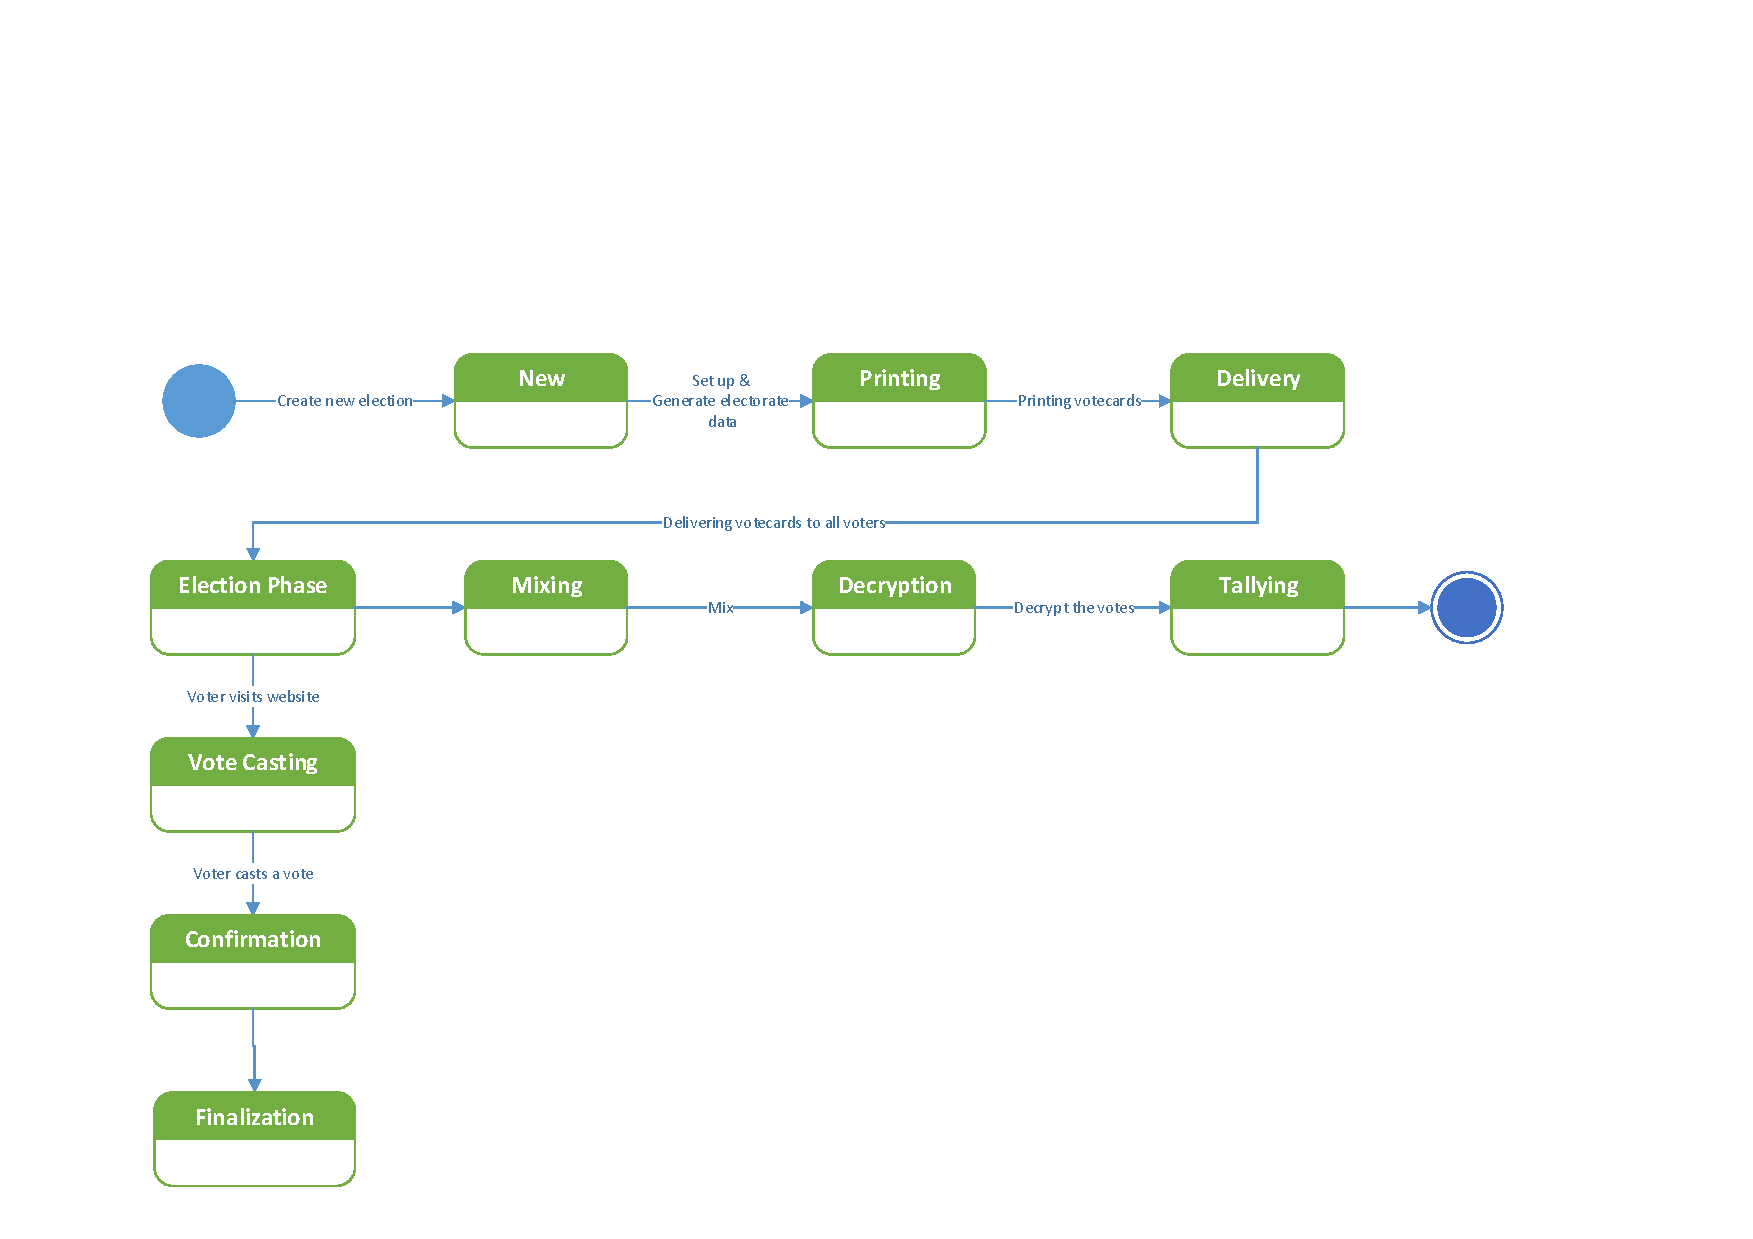
\includegraphics[scale=0.65]{assets/electionStatediagram.pdf}
\captionof{figure}{An election event consists of 7 different phases (green). During the election phase a voter can be in 3 different phases (blue)}\label{Phases of an election-event}%
\end{center}
\end{figure}

To give the users an opportunity to experience and gain insight into the functionality of the protocol a concept was implemented which enables them to take the perspective of every actor of the protocol at any given time and during each phase of the election event. This is why our application is divided into separate \textbf{views}, one for each actor:

Every actor involved in a CHVote election event has its own set of data to be displayed and specific tasks and use cases it has to perform. Most use cases are only available during a particular phase.

\begin{itemize}
	\item \textbf{Election Overview}: the election overview shows what phase the chosen election event is currently in. Additionally, a graphical schema shows how all the actors are connected and who is involved in the current phase.
\begin{figure}
\begin{center}
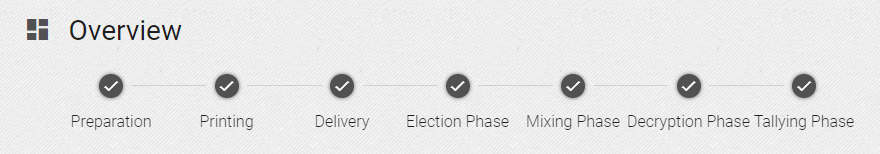
\includegraphics[scale=0.50]{assets/screenshots/overview.PNG}
\captionof{figure}{The election overview guides the user through the several phases of an election event and indicates which phases have been finished and what the next steps are.}\label{Election Overview}%
\end{center}
\end{figure}

	\item \textbf{Election Administrator View}: the view of the election administrator allows a user to set-up an election event by configuring the number of voters, the elections including the candidates and the number of selections per election. Instead of providing this information every time an election event is set up, previously defined election presets can be applied or the parameters can be generated randomly.

The election administrator view is also the place where the elections can be tallied and the final result is determined during the post-election phase.
	\item \textbf{Printing Authority View}: in the printing authority view, the voting cards can be printed and displayed for every voter. Additionally, the voting cards can be sent to the voters.

	\item \textbf{Election Authority View}: the election authority view first lets a user choose one of the three election authorities he wants to observe. On the top, new tasks will pop up whenever an election authority needs to perform a specific task, such as ballot or confirmation checking or mixing and decryption.

Additionally, the view shows the data that an election authority knows. This concept of dividing a view into tasks and data can be seen in figure \ref{Election Authority View} and has been used throughout the application in almost every view.

\begin{figure}[p]
\begin{center}
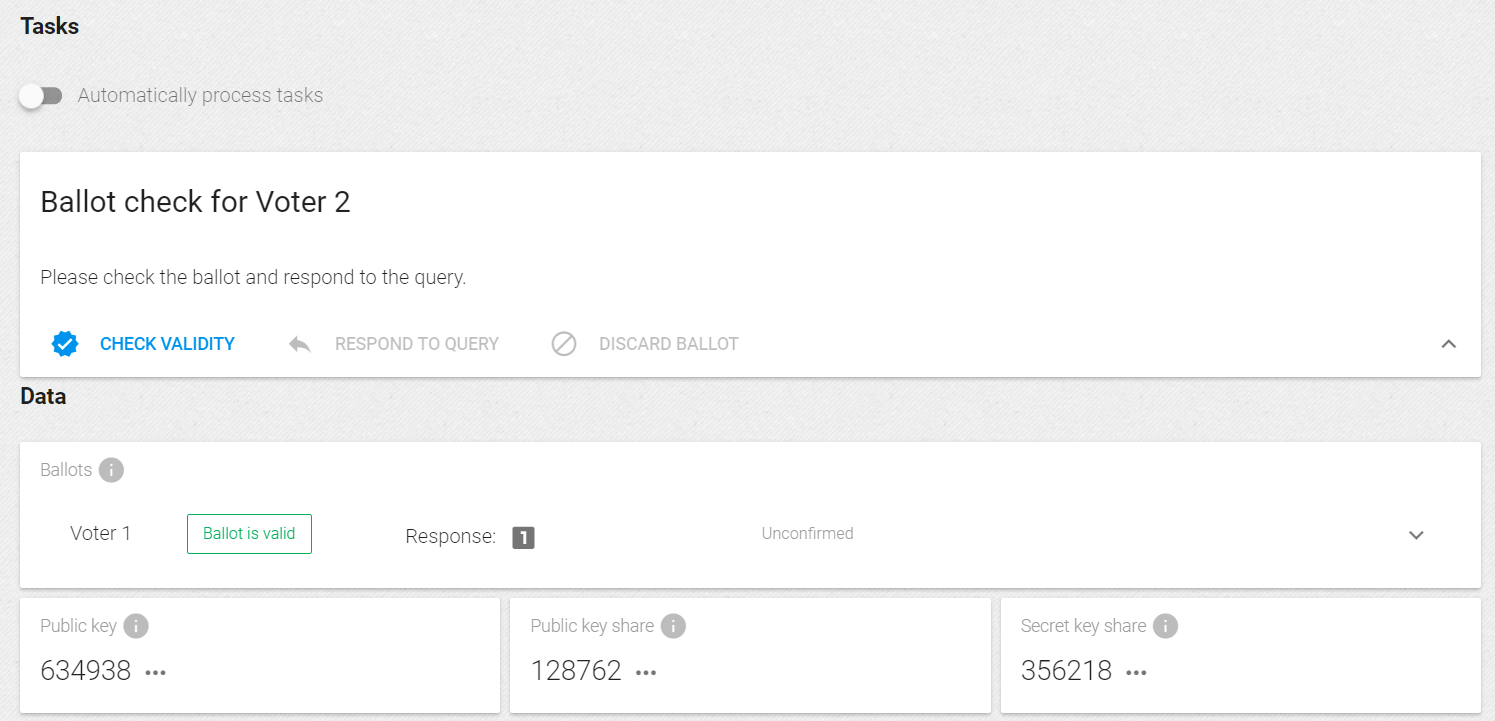
\includegraphics[scale=0.43]{assets/screenshots/view.png}
\captionof{figure}{The election authority view as an example of how the pages are generally structured: most views are divided into a tasks part which allows to perform the tasks of an actor, and a data part which shows what information about an election event the participant is in possession of. }\label{Election Authority View}%
\end{center}
\end{figure}

	\item \textbf{Voter View}: in the voter view, the vote casting process can be done for every voter that has been previously generated. The view displays both a voting form on the left and the voter's voting card on the right side. Two sensitive codes are hidden behind a scratchcard and can be copied to the voting card input by clicking on them after they have been revealed.

	\item \textbf{Bulletin Board View}: the bulletin board view always shows all the data that has been appended to the bulletin board by the other actors, such as the pre-election data, the ballots that the voters have cast, as well as all the proofs generated during the post-election phase.

	\item \textbf{Verifier View}: the view of the verifier becomes visible after the election result has been published to the bulletin board and the election event has reached its final stage. By clicking on the verify button, several checks are executed and the result is displayed on the page.
\end{itemize}

All the views are accessible from a tab view displayed on the top of the page which serves as the standard means of navigation, see figure \ref{Navigation}.

\begin{figure}[p]
\begin{center}
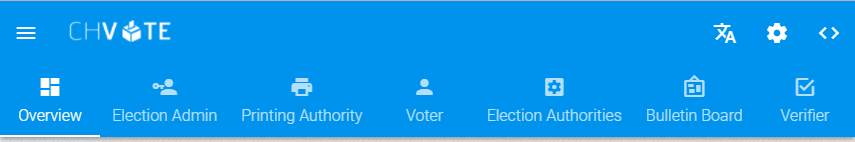
\includegraphics[scale=0.44]{assets/screenshots/navigation.png}
\captionof{figure}{The tab beyond the page header is the main control for navigating through the different pages. It also indicates where some interaction is required next by displaying an exclamation mark icon in the respective actor's tab.}\label{Navigation}%
\end{center}
\end{figure}

Based on the use cases, we tried to figure out all commonalities between the views: the views typically display the information known by the respective actor. Especially the bulletin board and election authorities could contain lots of information to be displayed. Most of the views have distinct tasks to be executed by the respective actor, such as casting a ballot in the voter's view or confirming ballots from an election authorities view.

The content that a view displays, or in other words, the functionality an actor has access to, depends on the phase the election event is currently in: during the pre-election phase the vote administrator needs to be able to set up the election, while in the tallying phase he must be able to tally and determine the final result.


\section{Design}
Given the rather large amount of complex data to be displayed, the main challenge of the project has been a well designed user interface which would allow to display all important information while maintaining a clear overview.

To achieve this goal we tried to keep our design very minimalistic and follow the Google material design guidelines as much as possible by choosing an appropriate UI component framework. Even though mobile compatibility was not a requirement, it was nevertheless our goal to make the layout as responsive as possible such that it could at least be used from a mobile phone, even though it was clearly optimized for desktop resolution.

Throughout the application we tried to establish common concepts regarding the look and feel and on how to display our data. Figure \ref{finalProduct} shows the consistency between our views in terms of the design and structure. One popular layout-concept of the Google material guidelines is the card layout. Cards can be easily integrated in a responsive grid system, look modern and allow to visually group data. In addition, we used pushover menus, tool-tips and pop-ups as they made it possible to hide less relevant information by default and display it only on demand of the user.

Before starting with the implementation of our application, we created mock-ups for most of the views to discuss our ideas with our supervisors and incorporated their feedback as well. The following screenshots are an extract of the mock-ups in which we tried to visualize how we imagined the resulting application would look like during the conceptual phase.

% Todo: Beispiel-Bild der Mockups %

Our conceptual work also involved developing a small prototype / proof of concept, in which we implemented one use case in a reduced extent with the envisaged frameworks and technologies to evaluate the technical feasibility. The next chapter covers in detail the languages and frameworks used in the project.

\begin{figure}
\begin{center}
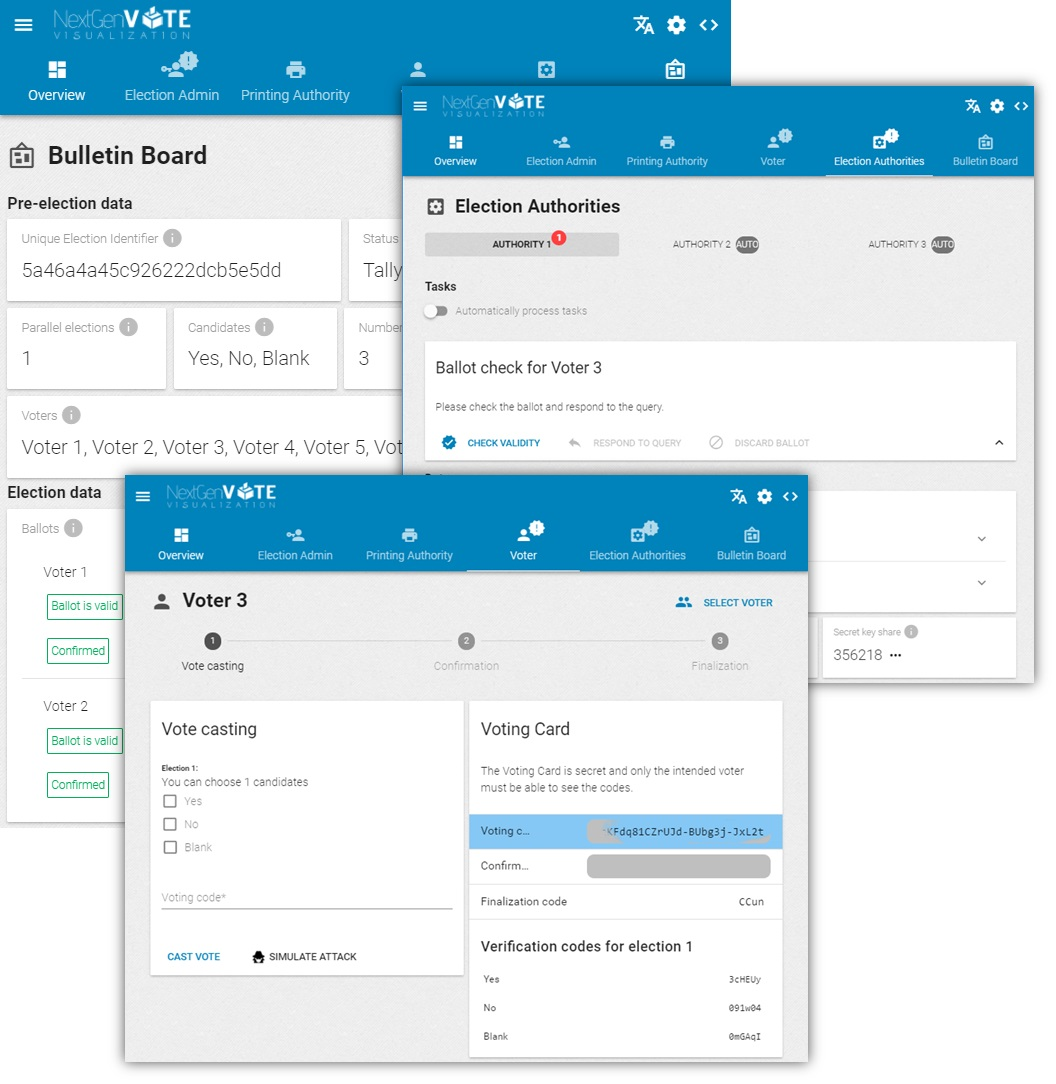
\includegraphics[scale=0.65]{assets/combined.png}
\captionof{figure}{Three views of our front-end, showing the consistent design and structure of our views }\label{finalProduct}%
\end{center}
\end{figure}
